
\section{Introduction}
\section{Motivation}
\section{Matrix formulation of the problem - 1D interferometer}

Here I intend to use convolution matrices properties to {\it qualitatively} study how ``pseudo-PSF'' vary as a
function of source location. Here I limit myselves to a 1-dimensional
interferometer (scalar only), so that
Convolution matrices are Toeplitz-symetyric (see bellow). In a more
general case, (along my intuition - but should be thought more
carefully), convolution matrices should be block-Toeplitz (each
block is a Toeplitz), while symetricity should still be true. 

\subsection{Remarks on the convolution and linear algebra}

In functional form the convolution theorem can be written as follows:


\def\F{\mathcal{F}}
\def\Fm{\bm{F}}
\def\Gauss{\bm{\mathcal{G}}}
\def\conv{\mathcal{*}}

\begin{alignat}{2}
%\label{eq:Lin}
%\F \left{ a.b\right}=&\F \left{ a\right}.\F \left{b\right}\\
\F \left\{  a.b\right\}=& \F \left\{a\right\}\conv\F \left\{b\right\}
\end{alignat}

Noting the convolution product is linear, we can reexpress the
convolution product and associated theorem asing linear
transformations:

\newcommand{\C}[1]{\bm{\mathcal{C}}_{#1}}
\newcommand{\vv}[1]{\bm{#1}}
\def\one{\bm{1}}


\begin{alignat}{2}
\label{eq:ConvTh}
%\F \left{ a.b\right}=&\F \left{ a\right}.\F \left{b\right}\\
\Fm \vv{A}\vv{b}=& \C{\vv{A}}\Fm \vv{b}
\end{alignat}

\noindent where $\Fm$ is the Fourier operator of size 
$n_{uv}\times n_{lm}$ ($\Fm$ is unitary $\Fm^H\Fm=\one$), $\vv{b}$ is
a vector with size $n_{lm}$. The matrix $\vv{A}$ models the scalar
multiplication of each point in $\vv{b}$, and is therefore diagonal of
size $n_{lm}\times n_{lm}$, and $\C{\vv{A}}$ is the convolution matrix
of size $n_{uv}\times n_{uv}$. There is a bijective relation

\begin{alignat}{2}
\label{eq:ConvTh}
%\F \left{ a.b\right}=&\F \left{ a\right}.\F \left{b\right}\\
\vv{A} \longleftrightarrow \C{\vv{A}}
\end{alignat}
 
\noindent in the sense that a scalar multiplucation defines a convolution
function and conversely. The matrices $\vv{A}$ and $\C{\vv{A}}$ always
have the following properties:

\begin{itemize}
  \item $\vv{A}$ is diagonal

   \item In the 1D case
\begin{itemize}
  \item $\C{\vv{A}}$ is Toeplitz
  \item In addition, for radiointerferometry, because the uv plane is symetric, $\C{\vv{A}}$ is symetric
\end{itemize}

\end{itemize}

The matrix $\C{\vv{A}}$ being Toeplitz, each row $\left[ \C{\vv{A}}
  \right]_l$ with sky coordinate $l$ can be built using a
rolling operator $\Delta_l$ that shifts the first row (the PSF at the field
center for example) to location of row $l$:

\begin{alignat}{2}
\label{eq:ConvTh}
%\F \left{ a.b\right}=&\F \left{ a\right}.\F \left{b\right}\\
\left[ \C{\vv{A}} \right]_l =& \Delta_l \left\{ \left[ \C{\vv{A}} \right]_0 \right\}
and&\\
\left[ \C{\vv{A}} \right]_0 =& \Fm^H \ \text{diag}(\vv{A})
\end{alignat}

The rolling operator is essentially just a reindexing, and has the
following properties:

\begin{alignat}{2}
\label{eq:PropsDelta0}
%\F \left{ a.b\right}=&\F \left{ a\right}.\F \left{b\right}\\
\Delta_l \left\{ a\vv{x} \right\} =&  a \Delta_l \left\{\vv{x} \right\} \\
\label{eq:PropsDelta1}
\Delta_l \left\{ \sum_i \vv{x}_i \right\} =& \sum_i \Delta_l \left\{ \vv{x}_i \right\} 
\end{alignat}

\newcommand{\roll}[1]{\Delta_l \left\{#1\right\}}


\subsection{PSF behaviour}

If $\vv{X}$ is the true sky, then the dirty image $\vv{X}^D_{ij}$ of
baseline $(ij)$ can be written as:

\begin{alignat}{2}
\vv{x}^D_{ij} =& \Fm^H \vv{S}_{c,ij}  \C{\vv{T}} \vv{S}_{\square,ij} \Fm \vv{A} \vv{x}
\end{alignat}

\noindent where $\vv{A}_{ij}$ models the DDE effets and is an
$n_{pix}\times n_{pix}$ diagonal matrix (taking polarisation into
account it is an
$4n_{pix}\times 4n_{pix}$ block diagonal matrix), $\vv{T}$ is the tapering/averaging function, 
$\vv{S}_{\square}$ samples the region over which the
tapering/averaging is made, and $\vv{S}_{c,ij}$ selects the central point
of the averaged/tapered visibility set. Using Eq. \ref{eq:ConvTh}, we have:

\begin{alignat}{2}
\vv{x}^D_{ij} =&\ \C{\vv{S}_{c,ij}}  \vv{T} \C{\vv{S}_{\square,ij}}  \Fm^H \Fm \vv{A}_{ij} \vv{x}\\ 
 =&\  \C{\vv{S}_{c,ij}}  \vv{T} \C{\vv{S}_{\square,ij}}  \vv{A}_{ij}  \vv{x}\\ 
\label{eq:approx}
 \sim&\  \C{\vv{S}_{c,ij}}  \vv{T}    \vv{A}_{ij} \vv{x}
\end{alignat}

\noindent where Eq. \ref{eq:approx} is true when the support of the
function $T$ is smaller than the sampling domain of
$\vv{S}_{\square}$. 

Averaged over all baselines, the dirty image becomes:

\begin{alignat}{2}
\label{eq:PPSF}
\vv{x}^D =&\bm{\mathcal{C}}_{STA} \vv{x}\\
\text{with }\bm{\mathcal{C}}_{STA}=&\sum_{ij}  \C{\vv{S}_{c,ij}}  \vv{T}    \vv{A}_{ij}
\end{alignat}



\subsection{Deriving the Pseudo-PSF}

\subsubsection{PSF and Pseudo-PSF}

{\bf We can already see that $\C{\vv{S}_{c,ij}}
  \vv{T}    \vv{A}_{ij}$ in Eq. \ref{eq:approx} is NOT Toeplitz anymore
  because each colunm is multiplied by a different value (DDE
  muliplied by the tapering function). The dirty sky is therefore not
  anymore the convolution of the true sky by the psf} {\it ie} the PSF
varies accross the field of view.

\subsubsection{Slow way}

Calculate the psf estimating $\mathcal{C}$ from direct
calculation. Eventually at discrete locations on a grid.


\subsubsection{Quickly deriving the Pseudo-PSF}

This is tricky part. The problem amount to finding any column $l$ of
$\bm{\mathcal{C}}$ on demand. For notation convenience, we merge
$\vv{T}$ and $\vv{A}_{ij}$ together in $\vv{A}_{ij}$. Operator
$\left[\vec{M}\right]_l$ extracts column $l$ from matrix $\vec{M}$,
and using Eq. \ref{eq:PropsDelta0}, \ref{eq:PropsDelta1} and \ref{eq:PPSF}:

\begin{alignat}{2}
\left[\bm{\mathcal{C}}\right]_l =&
     \left[\sum_{ij}  \C{\vv{S}_{c,ij}}  \vv{A}_{ij}\right]_l\\
=& \sum_{ij} a^l_{ij} \left[\C{\vv{S}_{c,ij}}\right]_l \\
&\ \ \ \text{with } a^l_{ij}=\vv{A}_{ij}(l)\\
=& \sum_{ij} \roll{a^l_{ij} \left[\C{\vv{S}_{c,ij}}\right]_0} \\
=& \sum_{ij} \roll{\Fm^H a^l_{ij}\ \text{diag}\left(\vv{S}_{c,ij}\right) }
\end{alignat}

If we now assume that at any given location $l$, the scalar $a^l_{ij}$
can be described by a smooth {\it function} of the uv coordinates
($(ij)$-indices), then we can write:

\begin{alignat}{2}
\left[\bm{\mathcal{C}}\right]_l =
& \sum_{ij} \roll{ \Fm^H \vv{A}^l\ \text{diag}\left(\vv{S}_{c,ij}\right) }\\
=& \sum_{ij} \roll{\C{\vv{A}^l}\ \Fm^H \text{diag}\left(\vv{S}_{c,ij}\right) }\\
=& \sum_{ij} \roll{\C{\vv{A}^l}\ \left[\C{\vv{S}_{c,ij}}\right]_0 }\\
=& \roll{\C{\vv{A}^l}\ \sum_{ij} \left[\C{\vv{S}_{c,ij}}\right]_0 }\\
=& \roll{\C{\vv{A}^l}\ \left[\C{\vv{S}_{c}}\right]_0 }\\
\end{alignat}

The approximate observed Pseudo-PSF is the convolution of the PSF at
the phase center ($\left[\C{\vv{S}_{c}}\right]_0$) and the fourier transform of the uv-dependent tapering function at given
lm ($\C{\vv{A}^l}$).

In other words, to compute the PSF at a given location $(lm)$:

\begin{itemize}
  \item Find $\vv{A}$:
    \begin{itemize}
    \item Compute weight $w_{ij}$ for each baseline $(ij)$
    \item Fit the uv-dependent weight by (for example), a Gaussian function $w_{ij}\sim w(u,v)=\Gauss\left(u,v\right)$ 
    \end{itemize}
  \item Compute the $PSF_{lm}$ at $(lm)$ from the PSF at the phase center $PSF_0$ as $PSF_{lm}=\mathcal{F}^{-1}\left(w\right)\conv PSF_0$
\end{itemize}
For example if the long baselines are more tapered, they are
"attenuated". The effective PSF on the edge of the field will get
larger by the convolution...
Something like that...
\section{Numerical Experiments}
We demonstrate the computational complexity of the quick, the slow derived PSF as a function of sky coordinates and 
perform a direct numerical results.
\subsection{Slow derivation}
\subsection{Quick derivation}
We will now show how to derived a pseudo PSF  which is based and resolved on the nominal PSF
but labelled by a set of band-limited integration.
In order to further optimize the slow derivation of the PSF described above to particularly reduce the computational
cost, we will need to understand the concept and theory of signal correlation in aperture synthesis.
It is worth noting in Radio Astronomy community that the cross-correlator output of two elements interferometer
in response to a source with spectral brightness distribution $I_{\nu}(\mathbf{s})$ as a function of the pointing direction $\mathbf{s}$ 
is the visibility function defined in Eq.\ref{eq:1} and obtained by integrating
over the solid angle $d\Omega$ \citep{thompson2008interferometry,taylor1999synthesis}
\begin{alignat}{2}
V_{}(\mathbf{b}) =& \int_{\Omega}I_{\nu}(\mathbf{s})e^{-2\pi i \mathbf{b}\mathbf{s}}d\Omega, \label{eq:1}
\end{alignat}
where $\mathbf{b}=\mathbf{b}(t,\nu)=(u_{t\nu}, v_{t\nu}, w_{t\nu})$  is the so called "\textit{baseline vector}" in wavelength
and with modulus the distance between the two elements
interferometer. The measurement in Eq.\ref{eq:1} is over the entire 
surface of the celestial sphere, practically the measurement is generally taken over a finite surface area of 
the celestial sphere due to the finite nature of the tracking source and other effects. Furthermore, the results is
averaged over finite time/frequency bins. Supose $\Delta t$ centered at $t_0$ and $\Delta \nu$ centered at $\nu_0$ the 
time and frequency averaged intervals respectively. 
Assuming that $\Delta t$ and  $\Delta \nu$ are small  enough so that $I_{\nu}(\mathbf{s})$
remains constant while the complex phase, $-2\pi i \mathbf{b}\mathbf{s}$ varies linearly.   Eq.\ref{eq:1} becomes:
\begin{alignat}{2}
V_{}(\mathbf{b}_0) =& \frac{1}{\Delta t \Delta \nu}\iint\limits_{\Delta t \Delta \nu}^{}W_{t_0,\nu_0}(t,\nu)\bigg[\int\limits_{\Omega}^{}I_{\nu}(\mathbf{s})e^{-2\pi i \mathbf{b}\mathbf{s}} d\Omega\bigg] dt d\nu \label{eq:2}\\	    
		    =& \iint\limits_{uv}^{}W_{\mathbf{b}_0}(\mathbf{b})\bigg[\int\limits_{\Omega}^{}I_{\nu}(\mathbf{s})e^{-2\pi i \mathbf{b}\mathbf{s}}d\Omega \bigg]du dv,  \label{eq:3}
\end{alignat}
where the following shorthand notation has been used.
\begin{alignat*}{2}
\hspace{-1cm}\mathbf{b}_0=&\mathbf{b}(t_0,\nu_0)\\
			 =&(u_{t_0\nu_0}, v_{t_0\nu_0}, w_{t_0\nu_0}),\\
\hspace{-1cm}W_{\mathbf{b}_0}(\mathbf{b})&=\frac{W_{t_0,\nu_0}(t,\nu)}{\Delta t \Delta \nu}.
\end{alignat*}
 Here, $\mathbf{b}_0$ is the baseline vector at centre
of a sampling interval and the sampling kernel $W_{\mathbf{b}_0}(\mathbf{b})$ is defined as:
\begin{alignat}{2}
W_{\mathbf{b}_0}(\mathbf{b})&=\Pi(\mathbf{b}-\mathbf{b}_0)w(\mathbf{b}-\mathbf{b}_0),
\end{alignat}
where, $\Pi(\mathbf{b}-\mathbf{b}_0)$ is a windowing function and $w(\mathbf{b}-\mathbf{b}_0)$ a weighting kernel.\\

As previously mentioned, we are interested on PSF's response. Therefore, Eq.\ref{eq:3} is restricted to the
complex visibility measured by the two elements interferometer for a point source located towards the direction 
$\mathbf{s}$ with unitary brightness. That said, $I_{\nu}(\mathbf{s})=\delta(\mathbf{b}_0)$ with $\delta$ the Dirac delta. 
It then follows that Eq\ref{eq:3} can be written as
\begin{alignat}{2}
V_{}(\mathbf{b}_0)  =& \iint\limits_{uv}W_{\mathbf{b}_0}(\mathbf{b})\mathbf{*}\delta(\mathbf{b}_0) e^{-2\pi i (u_{t\nu}l+v_{t\nu}m+w_{t\nu}(n-1))}du dv, \label{eq:4}
\end{alignat} 
The operator $*$ indicates convolution. Note that Eq.\ref{eq:4} is obtained after a
delay correction of $\mathbf{b}\mathbf{s_0}$ is  applied to the signals from the antennas 
array to steer towards the direction $\mathbf{s}_0$ and $\mathbf{b}(\mathbf{s}-\mathbf{s_0})=u_{t\nu}l + v_{t\nu}m + w_{t\nu}(n-1)$
describes the time difference between the two incoming signals. The three directions cosine $l,m$ and $n-1$ 
are  components of  $\mathbf{s}-\mathbf{s_0}$ given in radian with $n=\sqrt{1-l^2-m^2}$. For an extensive Discussion, see \citep{thompson2008interferometry,taylor1999synthesis}\\

Eq.\ref{eq:4} is two dimensional Fourier transform, making used of the convolution theorem which the litterature 
states that the Fourier transform of the product of two functions result to a convolution and vice-versa, the following
expansion is valid
\begin{alignat}{2}
V_{}(\mathbf{b}_0)  =& \mathcal{F}\Big\{W_{\mathbf{b}_0}(\mathbf{b})\Big\}\mathcal{F}\Big\{\delta(\mathbf{b}_0)\Big\} \\
		    =& \Bigg[\mathcal{F}\Big\{\Pi(\mathbf{b}-\mathbf{b}_0)\Big\}*\mathcal{F}\Big\{w(\mathbf{b}-\mathbf{b}_0)\Big\}\Bigg]\mathcal{F}\Big\{\delta(\mathbf{b}_0)\Big\}\\
		    =& C_{lm}(\mathbf{b}_0)\Bigg[\mathcal{F}\Big\{\Pi(\mathbf{b})\Big\}*\mathcal{F}\Big\{w(\mathbf{b})\Big\}\Bigg]\mathcal{F}\Big\{\delta(\mathbf{b}_0)\Big\}   \label{eq:5}
\end{alignat}
The symbol $\mathcal{F}$ denotes the Fourier transform and  $C_{lm}(\mathbf{b}_0)$ is obtained after we had apply the 
shifted Fourier transform properties. In other words, $C_{lm}(\mathbf{b}_0)$ is defined as
\begin{alignat*}{2}
C_{lm}(\mathbf{b}_0) &=e^{-2\pi i (u_{t_0\nu_0}l+v_{t_0\nu_0}m+w_{t_0\nu_0}(n-1))}
\end{alignat*}
% This expansion will be used to approximate the averaged or weighted averaged visibility
% $V_{}(\mathbf{b}_0)$.
If it is assumed that $\Pi(\mathbf{b})$ is the top-hat windowing function, then it can be demonstrated 
that its Fourier transform is (see Appendix A)
\begin{alignat*}{2}
\mathcal{F}\Big\{\Pi(\mathbf{b})\Big\}&=sinc\frac{-2\pi t\Delta \nu}{2}sinc\frac{-2\pi\nu\Delta t}{2}
\end{alignat*}
It is demonstrated in \citep{smirnov2011revisiting} that for  natural weighting, Eq.\ref{eq:5}  is approximated in term of the
phase changing in time $\Delta \Psi$ and frequency  $\Delta \Phi$ for the case of smearing as:
\begin{alignat*}{2}
V_{}(\mathbf{b}_0) &\simeq C_{lm}(\mathbf{b}_0)\Bigg[sinc\frac{\Delta \Psi}{2}sinc\frac{\Delta \Phi}{2}*\mathcal{F}\Big\{w(\mathbf{b}_0)\Bigg]\mathcal{F}\Big\{\delta(\mathbf{b}_0)\Big\}
%e^{-2\pi i (u_{t_c\nu_c}l+v_{t_c\nu_c}m+w_{t_c\nu_c}(n-1))}
\end{alignat*}
where $\Delta \Psi$ and $\Delta \Phi$ are explicitly defined as
\begin{alignat*}{2}
\Delta \Psi =&2\pi \Big[(u_{t_s\nu_0}-u_{t_e\nu_0})l + (v_{t_s\nu_0}-v_{t_e\nu_0})m\\
	    & +(w_{t_s\nu_0}-w_{t_e\nu_0})(n-1)\Big]\\
\Delta \Phi =&2\pi \Big[(u_{t_0\nu_s}-u_{t_0\nu_e})l + (v_{t_0\nu_s}-v_{t_0\nu_e})m\\
	    & +(w_{t_0\nu_s}-w_{t_0\nu_e})(n-1)\Big]
\end{alignat*}

We then generalized the approximation of smearing where $\Pi(\mathbf{b})$ is a radom windowing function 
as follows:
\begin{alignat*}{2}
V_{}(\mathbf{b}_0) &\simeq C_{lm}(\mathbf{b}_0)\Bigg[\mathcal{F}\Big\{\Pi(\mathbf{b}_0)\Big\}*\mathcal{F}\Big\{w(\mathbf{b}_0)\Big\}\Bigg]\mathcal{F}\Big\{\delta(\mathbf{b}_0)\Big\}
\end{alignat*}
\subsection{Imaging} 
Assuming that all the baselines are pointing at the same phase tracking centre, during conventional interferometric imaging,
the baseline visibilities are mapped on a uv-plane, and the result is inverse Fourier transformed:
\begin{alignat}{2}
PSF(\mathbf{s}) \simeq & \mathcal{F}^{-1}\Bigg\{\sum_{j=1}^{n_{bl}n_v}V_{pq}(\mathbf{b}_j)\Bigg\}\\
		\simeq & \mathcal{F}^{-1}\Bigg\{\sum_{j=1}^{n_{bl}n_v} C_{lm}(\mathbf{b}_0)\Bigg[\mathcal{F}\Big\{\Pi(\mathbf{b}_0)\Big\}\\
		&*\mathcal{F}\Big\{w(\mathbf{b}_0)\Big\}\Bigg]\mathcal{F}\Big\{\delta(\mathbf{b}_0)\Big\} \Bigg\}\\
		%\simeq & \sum_{pq,j=1}^{n_v}  \Bigg[\Pi(\mathbf{b}-\mathbf{b}_0)w(\mathbf{b}-\mathbf{b}_0)\Bigg] *\delta(\mathbf{b}_0)\\
		\simeq & \mathcal{C}(\mathbf{s})*PSF(\mathbf{s_0}),
\end{alignat}
where $PSF(\mathbf{s}_0)$ is the PSF at the phase tracking center
and $\mathcal{C}(\mathbf{s})$ is the image plane smearing response for a source
located toward the direction $\mathbf{s}\neq \mathbf{s_0}$. Note that, $n_v\times n_{bl}$ is the array 
total number of visibilities with $n_v$ and $n_{bl}$ the number of visibilities per 
baseline after approximation and the number of baselines respectively.





$\mathcal{C}(\mathbf{s})$ is defined as
\begin{alignat}{2}
\mathcal{C}(\mathbf{s}) &= \sum_{j=1}^{n_{bl}n_v}\mathcal{F}^{-1}\Big\{C_{lm}(\mathbf{b}_0)\Big\}*\Bigg[\Pi(\mathbf{b}_0)w(\mathbf{b}_0)\Bigg]
\end{alignat}



The smeared unnormalized PSF of a source, $PSF(\mathbf{s})$ located toward the
direction $\mathbf{s}$ was derived and shown that it is proportional
to the PSF, $PSF(\mathbf{s}_0)$ of a source at the phase centre.
% \begin{figure*}
% 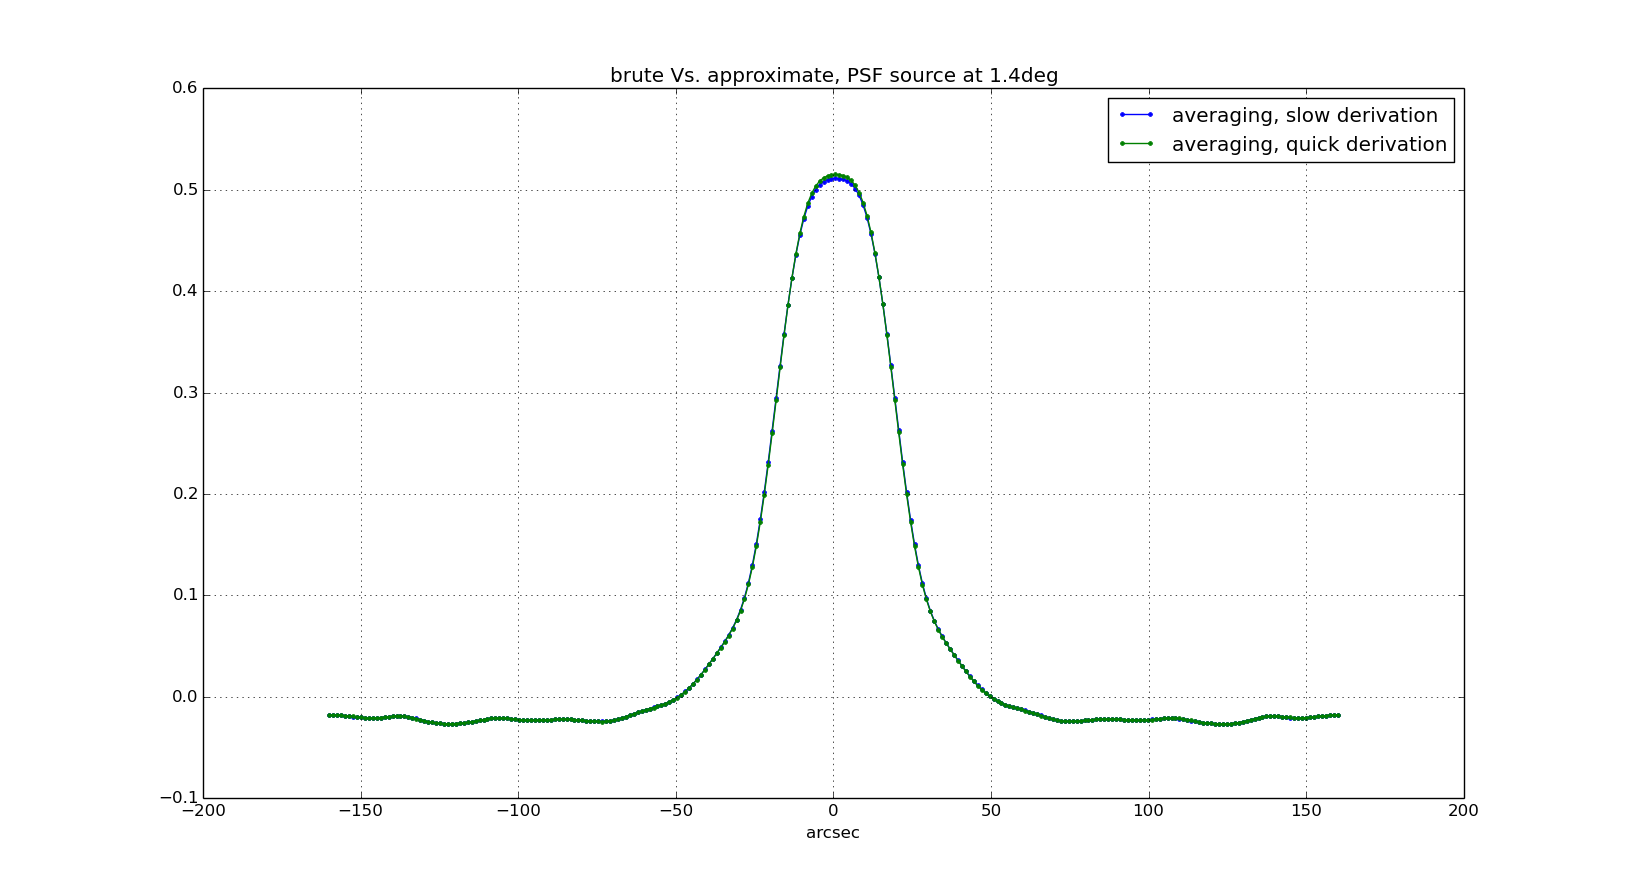
\includegraphics[width=1\textwidth]{./Figures/averaging_brute_quick_good.png}\caption{Brute Vs approximate PSF for a source at 1.4deg}\label{fig:uvcov}
%  \end{figure*}
%  \begin{figure*}
% 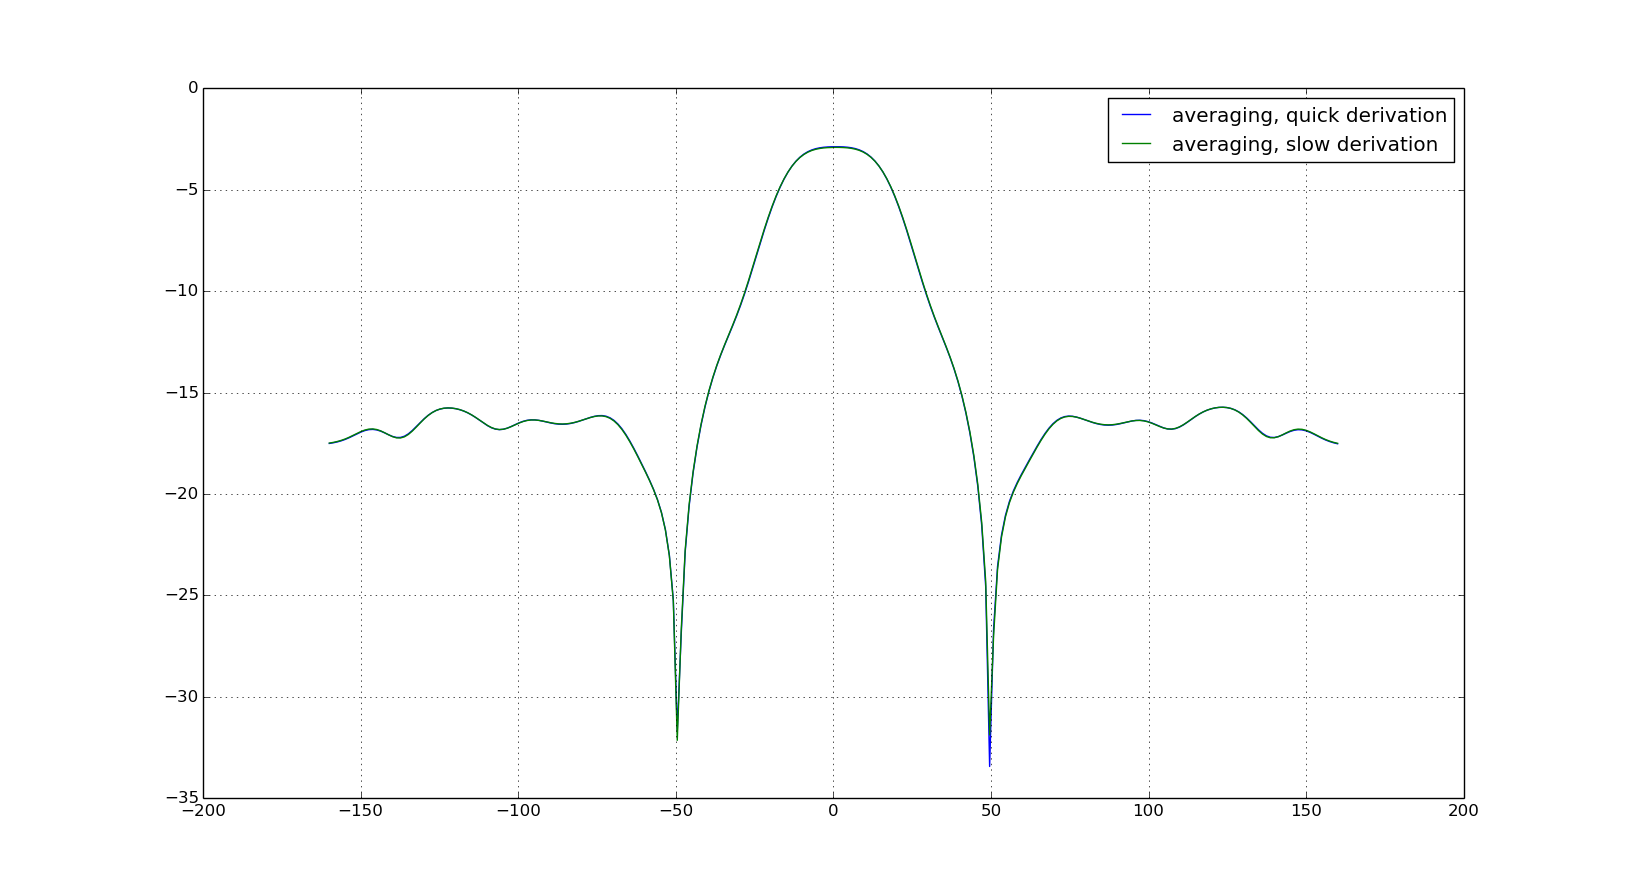
\includegraphics[width=1\textwidth]{./Figures/averaging_brute_quick_logscale.png}\caption{Brute Vs approximate PSF for a source at 1.4deg compare in log space}\label{fig:corrSigVLAMxBl_overlapGdelta}
% \end{figure*}
%  \begin{figure*}
% 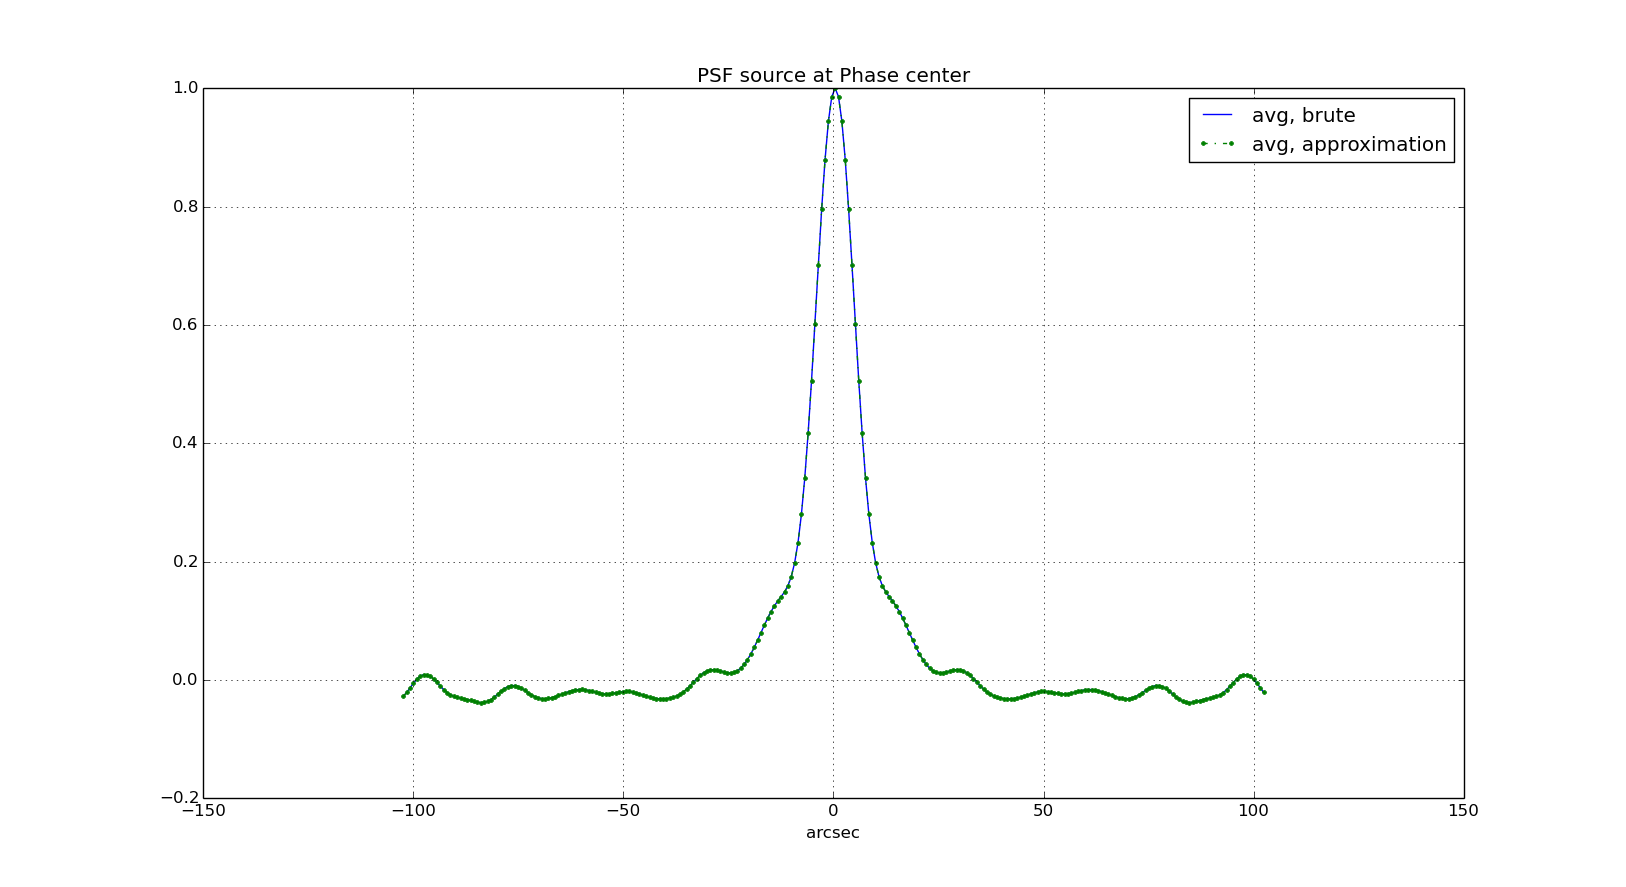
\includegraphics[width=1\textwidth]{./Figures/phasecentre.png}
% \end{figure*}

 \subsubsection{Computational cost} 
 \section{Simulation and comparison}
 \section{Discussion and conclusion}

